\documentclass{article}

% packages

\usepackage{setspace}
\usepackage{listings}
\usepackage{color}
\usepackage{graphicx}
\usepackage[dvipsnames]{xcolor}
\usepackage[hidelinks]{hyperref}
\usepackage[acronym]{glossaries}
\usepackage{fancyhdr}
%\usepackage{courier}
\usepackage{verbatim}
\usepackage{fancyvrb}
\usepackage{parskip}
\usepackage{tabularx}
\usepackage{ltablex}
\usepackage{array}
\usepackage{paralist}
\usepackage{titling}
\usepackage{xcolor}
\usepackage[
    left=0.80in,
    right=0.80in,
    top=1.0in,
    bottom=1.0in,
    paperheight=11in,
    paperwidth=8.5in
]{geometry}% 
\usepackage{rotating}

\geometry{a4paper}

\hypersetup{
    colorlinks,
    linkcolor={red!50!black},
    citecolor={blue!50!black},
    urlcolor={blue!80!black}
}

{\hyphenpenalty	10000}
\setlength{\parindent}{1cm} % Default is 15pt.

% new commands
% redefine itemsize: adds more vertical space between elements
\let\OLDitemize\itemize
\renewcommand\itemize{\OLDitemize\addtolength{\itemsep}{10pt}}
\definecolor{listingframecolor}{cmyk}{0,0,0,0.25}
\CustomVerbatimEnvironment{CodeListing}{Verbatim}{
  frame=single,
  rulecolor=\color{listingframecolor},
  framesep=6pt}
%\setlist{nosep}
\newcommand*{\includeCodeListing}[2][]{\VerbatimInput[
          frame=single,
          rulecolor=\color{listingframecolor},
  framesep=4pt,#1]{#2}}

\RecustomVerbatimCommand{\VerbatimInput}{VerbatimInput}%
{fontsize=\footnotesize,
 %
 %frame=lines,  % top and bottom rule only
 %framesep=2em, % separation between frame and text
 %rulecolor=\color{Gray},
 %commandchars=\|\(\), % escape character and argument delimiters for
                      % commands within the verbatim
 %commentchar=*        % comment character
}
\newcommand*{\textfile}[1]{\textsf{#1}}
\newcommand*{\textprog}[1]{\textfile{#1}}

\widowpenalties 1 10000
\raggedbottom

\newcommand{\code}[1]{\texttt{#1}}

\pagestyle{fancy}
%\fancyhead{}
% \lfoot{
%     \begin{minipage}[t][3px][b]{1cm}
%         \topskip0pt
%         \vspace*{\fill}
%         
\includegraphics[width=1cm]{pictures/epam-logo.png} 
%     \end{minipage}
% Nfstrace User and Developer Manual}
\fancyfoot[L]{Nfstrace User and Developer Manual}% \fancyfoot[R]{\thepage}
\renewcommand{\headrulewidth}{0.4pt}% Default \headrulewidth is 0.4pt
\renewcommand{\footrulewidth}{0.4pt}% Default \footrulewidth is 0pt
\rfoot{\today}

\makeglossaries

\lstset{frame=tb,
  language=Bash,
  aboveskip=3mm,
  belowskip=3mm,
  showstringspaces=false,
  columns=flexible,
  basicstyle={\small\ttfamily},
  numbers=none,
  numberstyle=\tiny\color{gray},
  keywordstyle=\color{blue},
  commentstyle=\color{dkgreen},
  stringstyle=\color{mauve},
  breaklines=true,
  breakatwhitespace=true,
  tabsize=3
}

%\pretitle{%
%  \begin{center}
%  \LARGE
%  
\includegraphics[width=3cm]{./pictures/epam-logo.png} 
%  \newline
%}
%\posttitle{\end{center}}
%\titlehead{
\includegraphics[width=3cm]{./pictures/epam-logo.png}}


% acronyms
\newacronym{BPF}{BPF}{Berkeley packet filter}
\newacronym{CIFS}{CIFS}{Common Internet File stem}
\newacronym{DPI}{DPI}{Deep Packet Inspection}
\newacronym{LSF}{LSF}{Linux Socket Filtering}
\newacronym{NFS}{NFS}{Network File System Protocol}
\newacronym{NIC}{NIC}{Network Interface Card}
\newacronym{POSIX}{POSIX}{Portable Operating System Interface for Unix}

% glossary entries 
\newglossaryentry{Gnuplot}
{
    name={Gnuplot},
    description={CLI tool that can generate two- and three-dimensional plots of data}
}
\newglossaryentry{Payload}
{
    name={Payload},
    description={User’s data transferred by NFS protocol. It is useless in analysis}
}
\newglossaryentry{rsize}
{
    name={rsize},
    description={option of NFS client connection to a NFS server}
}
\newglossaryentry{wsize}
{
    name={wsize},
    description={option of NFS client connection to a NFS server}
}
\newglossaryentry{Wireshark}
{
    name={Wireshark},
    description={Enterprise quality tool-set for network traffic analysis}
}

% ==============================================================================
\begin{document}
%\title{NFTRACE USER AND DEVELOPER MANUAL}

% Title begin 
% (titlepage is needed to display 
% image logo and title on the same page)
\begin{titlepage}

\newcommand{\HRule}{\rule{\linewidth}{0.5mm}} % Defines a new command for the horizontal lines, change thickness here


\includegraphics[width=2cm]{pictures/epam-logo.png}
\newline
\center
\vspace{3cm}

\includegraphics[width=5cm]{pictures/logo.png}

% \begin{tabular}{ l r }
% 
\includegraphics[width=2cm]{./pictures/epam-logo.png} &
%     \hspace{1cm} 
\includegraphics[width=5cm]{./pictures/logo.png} \\
% {\large \today}\\[2cm] & \\
% \end{tabular}
\par\vspace{1cm}
\center
{\huge NFSTRACE USER AND DEVELOPER MANUAL}\\[0.4cm] % Title of your document
{\centering {\small Version 0.4.0}} 
\vfill 
\end{titlepage} 
% Title end

%\maketitle 

\newpage

\vspace{5mm}
NFSTRACE User and developer manual 

\vspace{5mm}
EPAM Systems 

\vspace{5mm}
Copyright © 2014, 2015 EPAM Systems 

\vspace{5mm} This documentation is free software; you can redistribute it
and/or modify it under the terms of the GNU General Public License version 2 as
published by the Free Software Foundation.  

\vspace{5mm} This program is distributed in the hope that it will be useful,
but WITHOUT ANY WARRANTY; without even the implied warranty of MERCHANTABILITY
or FITNESS FOR A PARTICULAR PURPOSE. See the GNU General Public License for
more details.

\vspace{5mm} You should have received a copy of the GNU General Public License
along with this program; if not, write to the Free Software Foundation, Inc.,
51 Franklin Street, Fifth Floor, Boston, MA 02110-1301 USA.

\vspace{5mm} For more details see the file LICENSE in the source of nfstrace.

\vspace{5mm} This manual provides basic instructions on how to use \textprog{nfstrace} to
monitor \gls{NFS} and \gls{CIFS} activity and how to develop pluggable analysis
modules.

\newpage 

\tableofcontents

\newpage

\section{INTRODUCTION}

nfstrace performs live Ethernet 1 Gbps – 10 Gbps packets capturing and helps to
determine \gls{NFS} and \gls{CIFS} procedures in raw network traffic.
Furthermore, it performs filtration, dumping, compression, statistical
analysis, visualization and provides the API for custom pluggable analysis
modules. 

nfstrace captures raw packets from an Ethernet interface using libpcap
interface to Linux (\gls{LSF}) or FreeBSD (\gls{BPF}) implementations. At the
moment it is assumed that libpcap delivers correct TCP and UDP packets.
Assembling of IP packets from ethernet frames and IP packets defragmentation
are performed in the operating system's kernel.

The application has been tested on the workstations with integrated 1 Gbps
\gls{NIC}s (Ethernet 1000baseT/Full).

Currently \textprog{nfstrace} supports the following protocols:
\begin{CodeListing}
Ethernet | IPv4 | IPv6 | UDP | TCP |  NFSv3 | NFSv4 | NFSv4.1 | CIFSv1 | CIFSv2
\end{CodeListing}

\subsection{PORTABILITY}

The application has been developed and tested on GNU/Linux (Fedora 20, OpenSUSE
13.2, Ubuntu 14.04/14.10, CentOS 7, Arch Linux, Alt Linux 7.0.5) and FreeBSD
(FreeBSD 10.1). It is written in C++11 programming language and uses standard
\gls{POSIX} interfaces and the following libraries: libpthread, libpcap,
libstdc++.

\clearpage

\section{USAGE}
\subsection{OPTIONS}
\setlength\extrarowheight{3pt}
\begin{tabularx}{\linewidth}{ r X }
\textprog{-m}, & \code{--mode=live|dump|drain|stat} \\
 & Set the running mode (see the description below) (default: live).\\ 
\textprog{-i}, & \code{--interface=INTERFACE}\\
& Listen interface, it is required for live and dump modes (default: searches
for the lowest numbered, configured up interface (except loopback)).\\
\textprog{-f}, & \code{--filtration="filter"}\\
    & Specify the packet filter in \gls{BPF} syntax; for the expression syntax, see
pcapfilter(7) (default: "\code{port 2049 or port 445}").\\
\textprog{-s}, & \code{--snaplen=1..65535}\\
& Set the max length of captured raw packet (bigger packets will be truncated).
Can be used only for UDP (default: 65535).\\
\textprog{-t}, & \code{--timeout=milliseconds}\\
& Set the read timeout that will be used while capturing (default: 100).\\
\textprog{-b}, & \code{--bsize=MBytes}\\
& Set the size of the operating system capture buffer in MBytes; note that this
option is crucial for capturing performance (default: 20).\\
\textprog{-p}, & \code{--promisc}\\
& Put the capturing interface into promiscuous mode (default: true).\\
\textprog{-d}, & \code{--direction=in|out|inout}\\
& Set the direction for which packets will be captured (default: inout).\\
\textprog{-a}, & \code{--analysis=PATH\#opt1,opt2=val,...}\\
& Specify the path to an analysis module and set its options (if any).\\
\textprog{-I}, & \code{--ifile=PATH}\\
& Specify the input file for stat mode, '-' means stdin (default:
nfstrace\{filter\}.pcap).\\
\textprog{-O}, & \code{--ofile=PATH}\\
& Specify the output file for dump mode, '-' means stdout (default:
nfstrace-\{filter\}.pcap).\\ 
\textprog{--log}, & --log=PATH\\ & Specify the log file (default: nfstrace.log).\\
\textprog{-C}, & \code{--command="shell command"} \\
& Execute command for each dumped file.\\
\textprog{-D}, & \code{--dump-size=MBytes}\\
& Set the size of dumping file portion, 0 means no limit (default: 0).\\
\textprog{-E}, & \code{--enum=interfaces|plugins|-}\\
& Enumerate all available network interfaces and and/or all available plugins,
then exit; please note that interfaces can't be listed unless \textprog{nfstrace} was
built against the recent version of libpcap that supports the
pcap\_findalldevs() function (default: none).\\ 
\textprog{-M}, &
\textprog{--msg-header=1..4000}\\
& Truncate RPC messages to this limit (specified in bytes) before passing to a
pluggable analysis module (default: 512).\\
\textprog{-Q}, & \code{--qcapacity=1..65535}\\
& Set the initial capacity of the queue with RPC messages (default: 4096).\\
\textprog{-T}, & \code{--trace}\\
& Print collected NFSv3/NFSv4/NFSv4.1/CIFSv2 procedures, true if no modules were
passed with -a option.\\
\textprog{-Z}, & \code{--droproot=username}\\
& Drop root privileges after opening the capture device.\\
\textprog{-v}, & \code{--verbose=0|1|2}\\
& Specify verbosity level (default: 1).\\
\textprog{-h}, & \code{--help}\\
& Print help message and usage for modules passed with -a option, then exit.\\
\end{tabularx} 

\subsection{RUNNING MODES}

\begin{minipage}[t]{\linewidth}
\textprog{nfstrace} can operate in four different modes:
\vspace{5mm}
\begin{itemize}
\item online analysis (\textprog{--mode=live}): performs online capturing,
    filtration and live analysis of detected NFS/CIFS procedures using a
    pluggable analysis module or prints out them to stdout (\code{-T} or
    \code{--trace} options); \item online dumping (\textprog{--mode=dump}):
    performs online traffic capturing, filtration and dumping to the output
    file (specified with \code{-O} or \code{--ofile} options); 
\item offline analysis (\textprog{--mode=stat}):
    performs offline filtration of the .pcap that contains previously captured
    traces and performs analysis using a pluggable analysis module or prints
    found NFS/CIFS procedures to stdout (\code{-T} or \code{–trace} options); 
\item offline dumping (\textprog{--mode=drain}): performs a reading of traffic
    from the .pcap file (specified with \code{-I} or \code{--ifile} options),
    filtration, dumping to the output .pcap file (specified with \code{-O} or
    \code{--ofile} options) and removing all the packets that are not related
    to NFS/CIFS procedures.  \end{itemize}
\end{minipage}

\subsection{PACKETS FILTRATION}

Internally \textprog{nfstrace} uses libpcap that provides a portable interface to
the native system API for capturing network traffic. By so doing, filtration is
performed in the operating system's kernel. \textprog{nfstrace} provides a special option
(\code{-f} or \code{–-filtration}) for specifying custom filters in \gls{BPF} syntax.

The default \gls{BPF} filter in \textprog{nfstrace} is \textprog{port 2049 or port
445}, which means that each packet that is delivered to user-space from the
kernel satisfies the following conditions: it has IPv4 or IPv6 header and it
has TCP and UDP header with source or destination port number equals to 2049
(default NFS port) or 445 (default \gls{CIFS} port).

The reality is that this filter is very heavy and support of IPv6 is
experimental, so if you want to reach faster filtration of IPv4-only traffic we
suggest to use the following \gls{BPF} filter: \textprog{ip and port 2049 or port
445}.

\subsection{DUMP FILE FORMAT}
\label{sec:dumpfileformat}

\textprog{nfstrace} uses libpcap file format for input and output files so any
external tool (e.g. \gls{Wireshark}) can be used in order to inspect filtered
traces.

\subsection{USAGE EXAMPLES}

In this sections some use cases will be explained. Every next example inherit
something from the previous ones, so we suggest to read all of them from the
beginning.  

\subsubsection{AVAILABLE OPTIONS}

The following command demonstrates available options of the application and
plugged analysis modules (attached with \code{--analysis} or \code{-a} options). Note that
you can pass more than one module here.
\begin{CodeListing}
nfstrace –-help --analysis=libjson.so
\end{CodeListing}

\subsubsection{ONLINE TRACING}

The following command will run \textprog{nfstrace} in online analysis mode (specified with
\code{--mode} or \code{-m} options) without a pluggable analysis module. It will capture
\gls{NFS} traffic transferred over TCP or UDP with source or destination port
number equals to 2049 and will simply print them out to stdout (\code{-T} or \code{--trace}
options). Capturing is over when \textprog{nfstrace} receives \textprog{SIGINT} (Control-C).  Note
that capturing from network interface requires superuser privileges.

\begin{CodeListing} 
nfstrace -–mode=live --filtration="ip and port 2049" -T 
\end{CodeListing}

\subsubsection{ONLINE ANALYSIS}

The following command demonstrates running \textprog{nfstrace} in online analysis mode.
Just like in the previous example it will capture \gls{NFS} traffic transferred
over TCP or UDP with source or destination port number equals to 2049 and then
it will perform Operation Breakdown analysis using pluggable analysis module
\code{libbreakdown.so}.
\begin{CodeListing}
nfstrace –-mode=live -–filtration=”ip and port 2049” --analysis=libbreakdown.so
\end{CodeListing}

\subsubsection{ONLINE DUMPING AND OFFLINE ANALYSIS}

The following example demonstrates running \textprog{nfstrace} in online
dumping and offline analysis modes.  At first \textprog{nfstrace} will capture
\gls{NFS} traffic transferred over TCP or UDP with source or destination port
number equals to 2049 and will dump captured packets to \code{dump.pcap} file
(specified with \code{--ofile} or \code{-O} options).  At the second run
\textprog{nfstrace} will perform offline Operation Breakdown analysis using
pluggable analysis module \code{libbreakdown.so}.  \begin{CodeListing}
\# Dump captured packets to dump.pcap 
nfstrace --mode=dump
         --filtration="ip and port 2049"
         -O dump.pcap 
\# Analyse dump.pcap using libbreakdown.so 
nfstrace --mode=stat
         -I dump.pcap
         --analysis=libbreakdown.so
\end{CodeListing}

\subsubsection{ONLINE DUMPING, COMPRESSION AND OFFLINE ANALYSIS}

The following example demonstrates running \textprog{nfstrace} in online dumping and
offline analysis modes. Since dump file can easily exhaust disk space,
compression makes sense.

At first \textprog{nfstrace} will capture \gls{NFS} traffic transferred over TCP or UDP
with source or destination port number equals to 2049 and will dump captured
packets to \code{dump.pcap} file.

Note that compression is done by the external tool (executed in script passed
with \code{--command} or \code{-C}  options) and it will be executed when
capturing is done.  The output file can be inspected using some external tool
as described in \ref{sec:dumpfileformat}.

At the second run \textprog{nfstrace} will perform offline analysis. Again, the external
tool (bzcat in this example) is used in order to decompress previously saved
dump. \textprog{nfstrace} will read \code{stdin} (note the \code{-I -} option) and perform offline
analysis using Operation Breakdown analyzer.

\begin{CodeListing}
\# Dump captured procedures to dump.pcap file.
\# Compress output using bzip2 when capturing is over. 
nfstrace --mode=dump
         --filtration="ip and port 2049"
         -O dump.pcap
         -C "bzip2 -f -9"
\# Extract dump.pcap from dump.pcap.bz2 to stdin.
\# Read stdin and analyze data with libbreakdown.so module. 
bzcat dump.pcap.bz2 | nfstrace --mode=stat
                               -I -
                               --analysis=libbreakdown.so
\end{CodeListing}

\subsubsection{ONLINE DUMPING WITH FILE LIMIT, COMPRESSION AND OFFLINE ANALYSIS}

This example is similar to the previous one except one thing: output dump file
can be very huge and cause problems in some situations, so \textprog{nfstrace} provides
the ability to split it into parts.

At first \textprog{nfstrace} will be invoked in online dumping mode. Everything is similar
to the previous example except \code{-D} (\code{--dump-size}) option: it specifies the size
limit in MBytes, so dump file will be split according to this value.

At the second run \textprog{nfstrace} will perform offline analysis of captured packets
using Operation Breakdown analyzer.

Please note that only the first dump file has the pcap header.

\begin{CodeListing}
\# Dump captured procedures to the multiple files and compress them. 
nfstrace --mode=dump \
         --filtration="ip and port 2049" \
         -O dump.pcap \
         -D 1 \
         -C "bzip2 -f -9"

\# get list of parts in the right order:
\#    dump.pcap.bz2
\#    dump.pcap-1.bz2
parts=\$(ls dump.pcap*.bz2 | sort -n -t - -k 2)
\# Extract main dump.pcap and parts from dump.pcap.bz2 to stdin.
\# Read stdin and analyze data with libbreakdown.so module. 
bzcat “\$parts” | nfstrace --mode=stat
-I -
--analysis=libbreakdown.so
\end{CodeListing}

\subsubsection{VISUALIZATION}
\label{sec:visualization}

This example demonstrates the ability to plot graphical representation of data
collected by Operation Breakdown analyzer.

\code{nst.sh} is a shell script that collects data generated by analyzers and
passes it to \gls{Gnuplot} script specified with -a option.  

\code{breakdown\_nfsv3.plt} and \code{breakdown\_nfsv4.plt} are a \gls{Gnuplot}
scripts that understand output data format of Operation Breakdown analyzer and
generate .png files with plots.  Note that \gls{Gnuplot} must be installed.

\begin{minipage}[t]{\linewidth}
\begin{CodeListing}
# Extract dump.pcap from dump.pcap.bz2 to stdin.
# Read stdin and analyze data with libbreakdown.so module. 
bzcat trace.pcap.bz2 | nfstrace -m stat -I - -a libbreakdown.so

# Generate plot according to *.dat files generated by
# libbreakdown.so analyzer. 
nst.sh -a breakdown.plt -d . -p 'breakdown*.dat' -v
\end{CodeListing} 
\end{minipage}

\section{ANALYZERS}

All pluggable modules are implemented as external shared libraries.

\subsection{OPERATION BREAKDOWN ANALYZER (LIBBREAKDOWN.SO)}

Operation Breakdown (OB) analyzer calculates average frequency of NFS/CIFS
procedures and computes standard deviation of latency.

\begin{CodeListing} 
\$ nfstrace -a libbreakdown.so –h
nfstrace 0.4.0 (Release) built on Linux-3.16.1-1-generic by C++ compiler GNU 4.9.1 
Usage: ./nfstrace [OPTIONS]... 
\end{CodeListing}
And the result of execution will look something like this:
\includeCodeListing{nfstrace_manual_includes/breakdown_output.txt}
%\begin{CodeListing}
%\end{CodeListing}
OB analyzer produces \code{.dat} file in the current directory for each detected
NFS/CIFS session:
\begin{CodeListing}
$ ls -a *.dat breakdown\_10.6.137.79:949 --> 10.6.7.38:2049 [TCP].dat
\end{CodeListing} 
As described in \ref{sec:visualization}, produced \code{.dat}
files can be visualized using \code{nst.sh} and \code{breakdown\_nfsv3.plt} or
\code{breakdown\_nfsv4.plt} (according to \gls{NFS} version).
\begin{CodeListing} 
nst.sh -a breakdown\_nfsv3.plt -d . -f 'breakdown\_10.6.137.79:949 -->
10.6.7.38:2049 [TCP].dat' 
\end{CodeListing}

\begin{figure}
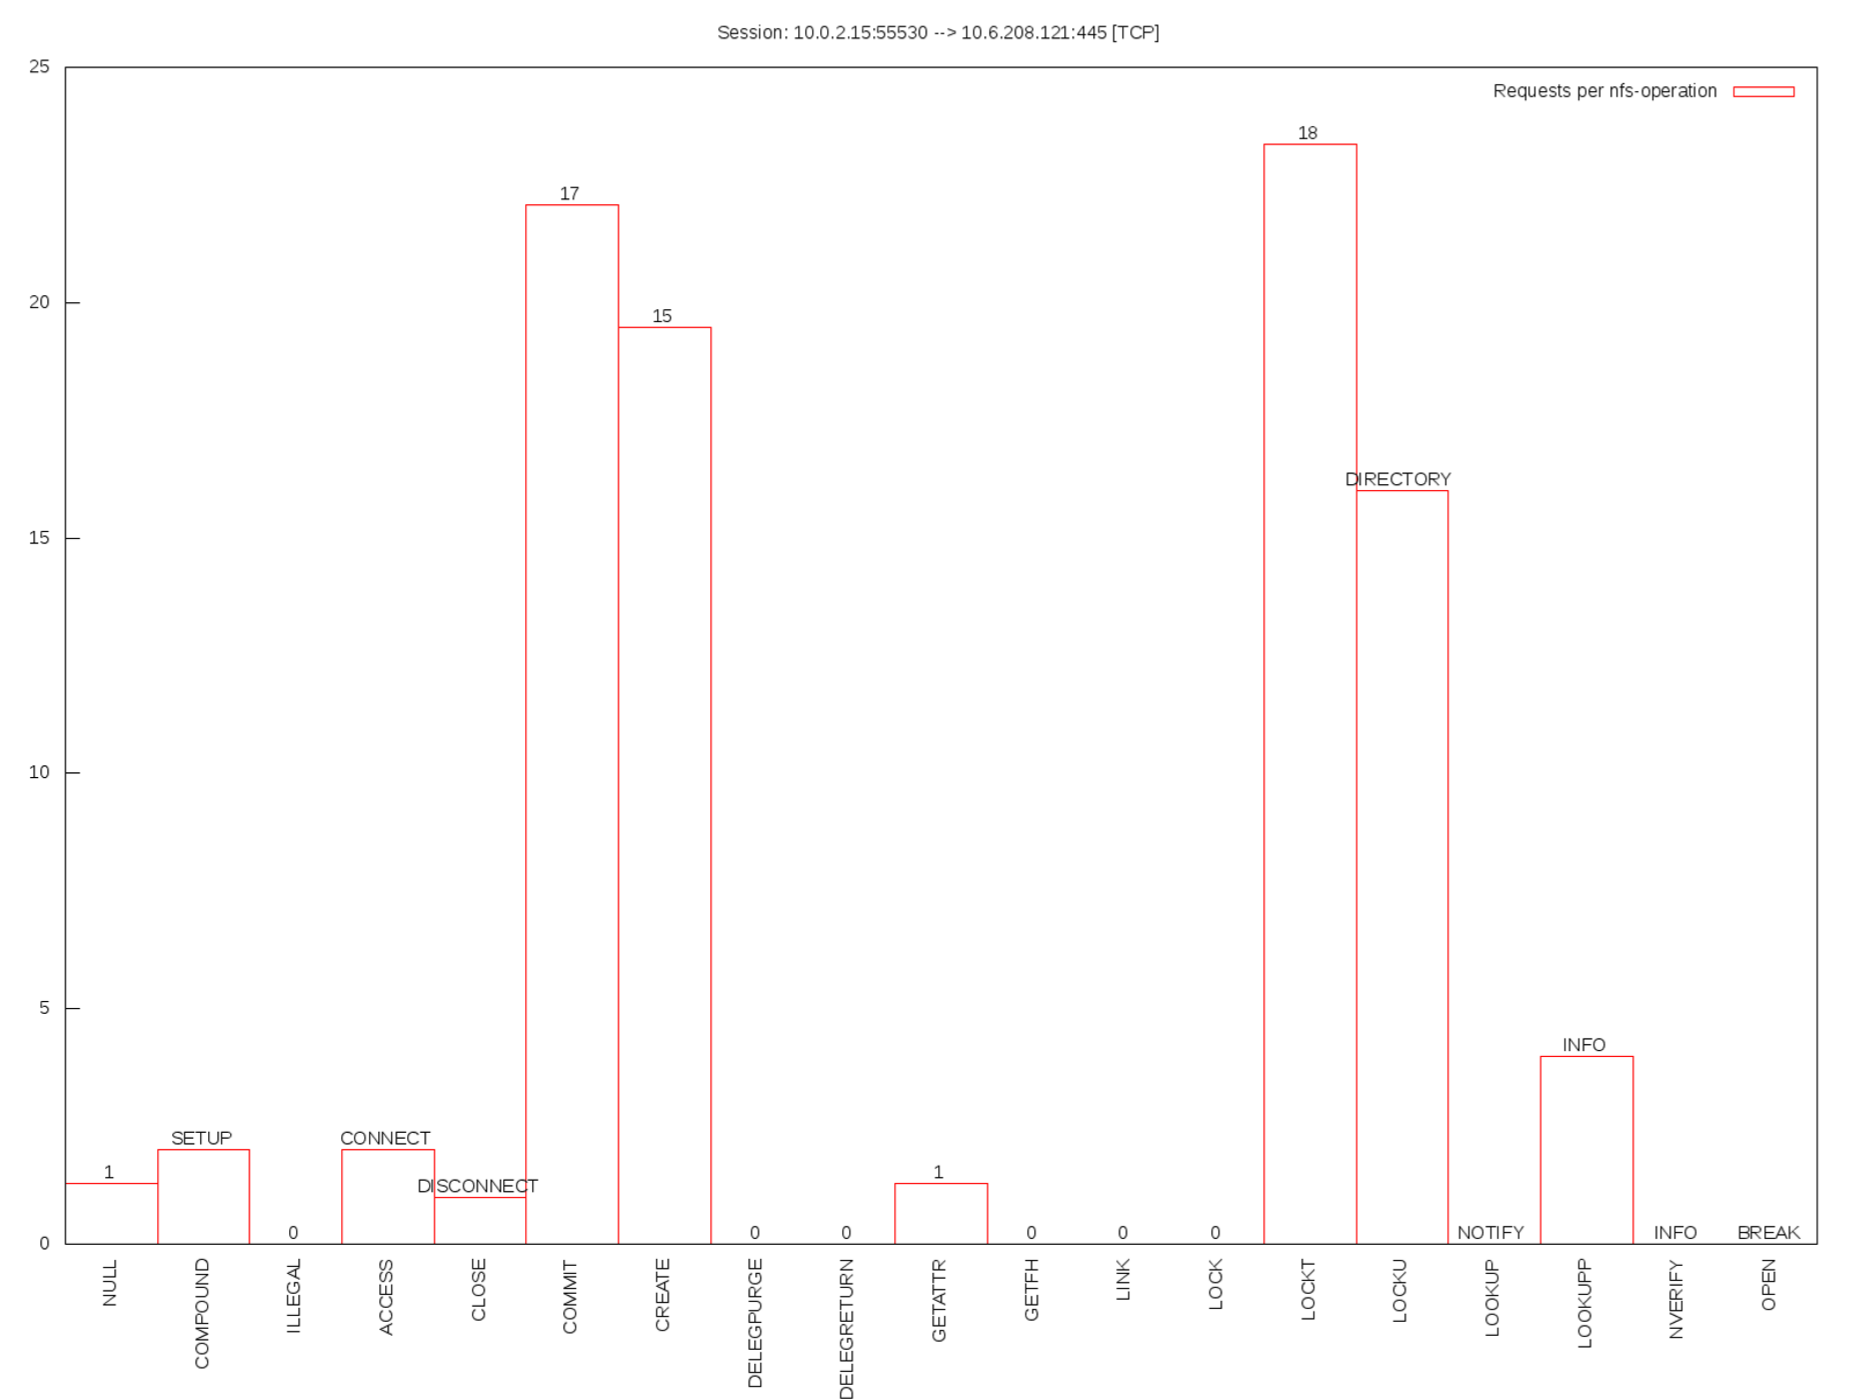
\includegraphics[width=\linewidth]{./pictures/session-visualization.png}
\caption{Session visualization}
\label{Session visualization}
\centering
\end{figure}

\subsection{WATCH (LIBWATCH.SO)}

Watch plugin mimics old nfswatch utility: it monitors \gls{NFS} and \gls{CIFS}
traffic and displays it in terminal using \code{ncurses}. It supports NFSv3, NFSv4,
NFSv4.1, CIFSv1 and CIFSv2.

\begin{minipage}[t]{\linewidth}
\includeCodeListing{nfstrace_manual_includes/libwatch_output.txt} 
\end{minipage}

\vspace{5mm}

By default watch plugin will update its screen every second, you can specify
another timeout in milliseconds:

\begin{CodeListing}
$ nfstrace -a libwatch.so#2000
\end{CodeListing}

\subsection{JSON ANALYZER (LIBJSON.SO)}
JSON analyzer calculates a total amount of each supported application protocol
operation. It accepts TCP-connections on particular TCP-endpoint (host:port),
sends a respective JSON to the TCP-client and closes connection. Suggested to
be used in live mode.

Available options:

\begin{minipage}[t]{\linewidth}
\begin{tabular}{ll}
\textprog{host=HOSTNAME} &
Network interface to listen (default: listen all interfaces)\\
\textprog{port=PORT} &
IP-port to bind to (default: 8888)\\
\textprog{workers=WORKERS} &
Amount of worker threads (default: 10)\\
\textprog{duration=DURATION} &
Max serving duration in milliseconds (default: 500)\\
\textprog{backlog=BACKLOG} &
Listen backlog (default: 15)\\
\end{tabular}
\end{minipage}

In order to try this analyzer out you can start \textprog{nfstrace} in on terminal:
\begin{CodeListing}
$ nfstrace -i eth0 -a libjson.so\#host=localhost
\end{CodeListing}
And then you can make a TCP-request to \textprog{nfstrace} in another terminal to fetch
current statistics:

\begin{minipage}[t]{\linewidth}
\includeCodeListing{nfstrace_manual_includes/telnet_output.txt} 
\end{minipage}

\section{IMPLEMENTATION DETAILS}

This section may be interested for the developers who want to contribute or
implement new pluggable analysis module.

\subsection{PAYLOAD FILTRATION}

Each NFSv3 procedure consists of two RPC messages:

\begin{itemize}
    \item call – request from client to server;
    \item reply – reply from server with result of requested procedure.
\end{itemize}
\vspace{5mm}

Both RPC messages may contain data useful for analysis. Both RPC messages may
contain thousands of \gls{Payload} bytes useless for analysis. nfstrace
captures headers of calls and replies and then matches pairs of them to
complete \gls{NFS} procedures.

The \code{--snaplen} option sets up the amount of bytes of incoming packet for
uprising from the kernel to user-space. In case of TCP transport layer this
option is useless because TCP connection is a bidirectional stream of data
(instead of UDP that is form of interchange up to 64k datagrams). In case of
\gls{NFS} over TCP \textprog{nfstrace} captures whole packets and copies them to
user-space from the kernel for \gls{DPI} and performing \gls{NFS} statistical
analysis.

Finally, \textprog{nfstrace} filtrates whole \gls{NFS} traffic passed from the kernel to
user-space and detects RPC/NFS message headers (up to 4 Kbytes) within
gigabytes of network traffic.

Detected headers are copied into internal buffers (or dumped into a
\code{.pcap} file) for statistical analysis.

The key principle of the filtration here is \textbf{discard \gls{Payload}
ASAP}.

Filtration module works in a separate thread and captures packets from network
interface using libpcap. It matches packets to a related session (TCP or UDP)
and performs reassembling of TCP flow from a TCP segment of a packet. After
that the part of a packet will be passed to \code{RPCFiltrator}. In case of NFSv4 the
whole packet will be passed to \code{RPCFiltrator} because it consists of several
NFSv4 operations.  

There are two \code{RPCFiltrator} in one TCP session. Both of them
know the state of the current RPC message in related TCP flow. They can detect
RPC messages and perform actions on a packet: discard it or collect for
analysis.

The size of the kernel capture buffer can be set with \code{-b} option (in
MBytes).  Note that this option is very crucial for capturing performance.

\gls{wsize} and \gls{rsize} of an \gls{NFS} connection are important for
filtration and performance analysis too.

\subsection{PLUGGABLE ANALYSIS MODULES}

nfstrace provides C++ api for implementing pluggable analysis modules. Header
files provide definitions of \code{IAnalyzer} interface, NFS/CIFS data structures and
functions. The \code{IAnalyzer} interface is a set of NFS/CIFS handlers that will be
called by \code{Analysis} module for each NFS/CIFS procedure. All constants and
definitions of types will be included with \code{<nfstrace/api/plugin\_api.h>} header.

A pluggable analysis module must be a dynamically linked shared object and must
export the following C functions:

\begin{CodeListing}
const char* usage (); // return description of expected opts for create(opts)
IAnalyzer* create (const char* opts); // create and return an instance of an Analyzer 
void destroy (IAnalyzer* instance); // destroy created instance of an Analyzer 
const AnalyzerRequirements* requirements(); // return Analyzer's requirements 
\end{CodeListing}
After the declaration of all these function there must be the following macro:
\begin{CodeListing}
NST_PLUGIN_ENTRY_POINTS (&usage, &create, &destroy, &requirements)
\end{CodeListing}

\textprog{usage()} function must return a C-string with module description and
required parameters for creation of an instance of analyzer, this string will
be shown in the output of \code{--help} option.

\textprog{IAnalyzer* create(const char* opts)} must create and return an instance
of the analyzer according to passed options.  

\textprog{void destroy(IAnalyzer* instance)} must destroy previously created
analyzer instance and perform required cleanups (e.g. close connection to a
database etc.).

\textprog{const AnalyzerRequirements* requirements()} must create and return an
instance of analyzer requirements. Its silence property is used if exclusive
control over standard output is required.

All existing analyzers are implemented as pluggable analysis modules and can be
attached to \textprog{nfstrace} with \code{-a} option.

\subsection{GENERAL SCHEMA}

\begin{minipage}[t]{\linewidth}
The general schema of \textprog{nfstrace} is presented in the Figure \ref{fig:generalschema}.
In this schema you can see how data flows in different modes: 
\begin{itemize}
    \item on-line analysis –  \colorbox{green}{green line}
    \item on-line dumping –  \colorbox{yellow}{yellow line}
    \item off-line dumping –  \colorbox{ProcessBlue}{blue line}
    \item off-line analysis –  \colorbox{orange}{orange line}
\end{itemize} 
\end{minipage}

\newpage

\begin{sidewaysfigure}
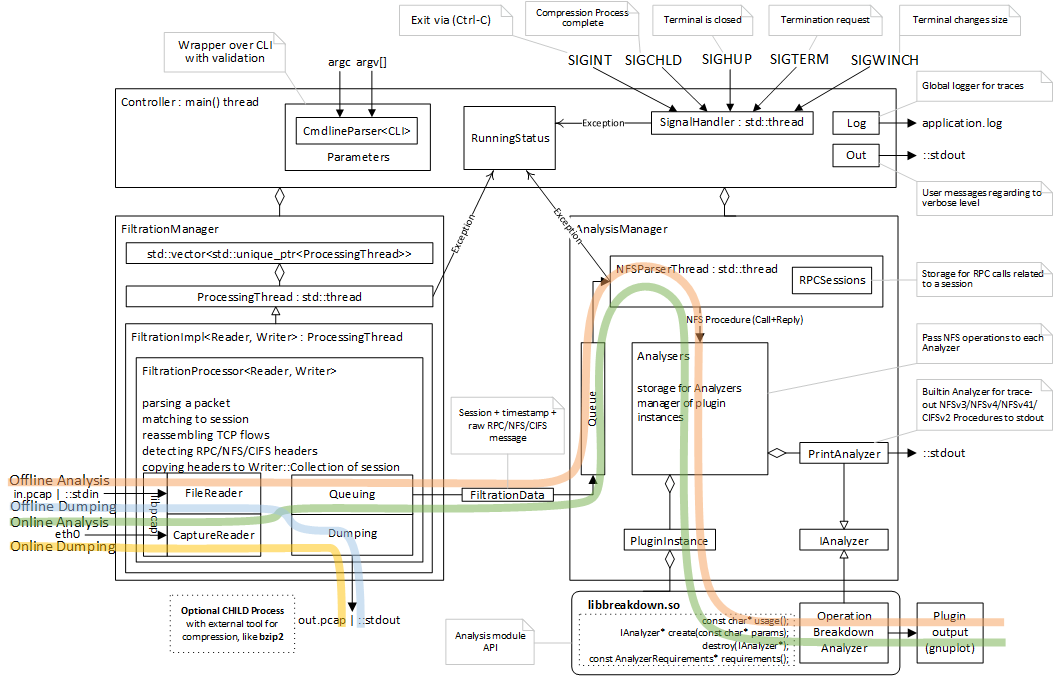
\includegraphics[width=\linewidth]{./pictures/general-structure.png}
\caption{General schema}
\label{General schema}
\centering
\label{fig:generalschema}
\end{sidewaysfigure}

\clearpage

\printglossaries 

\end{document}
